\documentclass{article}

\renewcommand{\refname}{Referencias}

\usepackage[colorlinks=true, urlcolor=blue, linkcolor=black]{hyperref}

\usepackage{amsmath} % \usepackage is a command that allows you to add functionality to your LaTeX code
\usepackage{graphicx}
\graphicspath{{./assets/}}

\title{Desafío 2: Análisis forense digital} % Sets article title
\author{Tomas Santana - C.I. 30 604 530} % Sets authors name

\date{2 de Julio de 2024} % Sets date
\setlength{\parskip}{.5\baselineskip}

\begin{document}
\maketitle
\section{Introducción}
Durante este desafío, se buscará analizar y resolver los retos dejados por el atacante en la máquina \texttt{URU-Challenge-2}, utilizando técnicas de análisis criptográfico y de análisis de tráfico de red. El presente informe documenta las acciones llevadas a cabo para resolver los retos propuestos.

\section{Reconocimiento}
\subsection{Ingreso a la máquina}

En este caso, la obtención de acceso fue muy sencilla, ya que se nos propocionó con el usuario y contraseña de interés. Se estableció una conexión SSH con la máquina utilizando el comando que se muestra en la Figura \ref{fig:ssh}.

Con esto, se obtuvo acceso a la máquina y se pudo comenzar a analizar los archivos y servicios que se encontraban en ella.

\begin{figure}[ht!]
  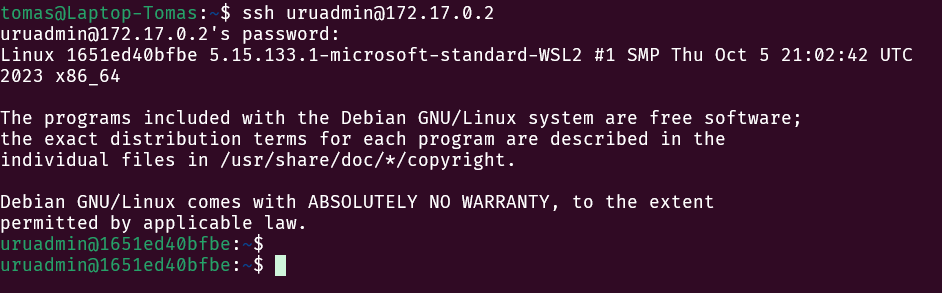
\includegraphics[width=\textwidth]{ssh.png}
  \caption{Conexión SSH a la máquina \texttt{URU-Challenge-2}}
  \label{fig:ssh}
\end{figure}

\subsection{Exploración de archivos}

Este paso también fue sencillo, ya que la descripción del problema indicó que los archivos de interés se encuentran en el directorio \texttt{/home/uruadmin}. Un simple comando \texttt{ls} nos permitió ver los archivos que se encontraban en el directorio, y se pudieron identificar cuatro archivos de interés. Se pueden ver los archivos en la Figura \ref{fig:ls}.

\begin{figure}[ht!]
  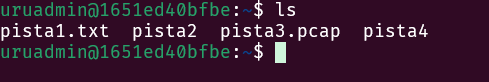
\includegraphics[width=\textwidth]{ls.png}
  \caption{Archivos en el directorio \texttt{/home/uruadmin}}
  \label{fig:ls}
\end{figure}

\section{Análisis de pistas}

\subsection{Archivo 1: \texttt{pista1.txt}}

Imprimiendo los contenidos de este archivo con el comando \texttt{cat}, se obtuvo el resultado que se muestra en la Figura \ref{fig:pista1}. Se puede ver que el contenido es una cadena de texto cifrada. Como respeta una secuencia de caracteres similar a la del texto escrito (en cuanto a espacio y longitud de palabras), se puede inferir que es un tipo de cifrado clásico, como sustitución.

\begin{figure}[ht!]
  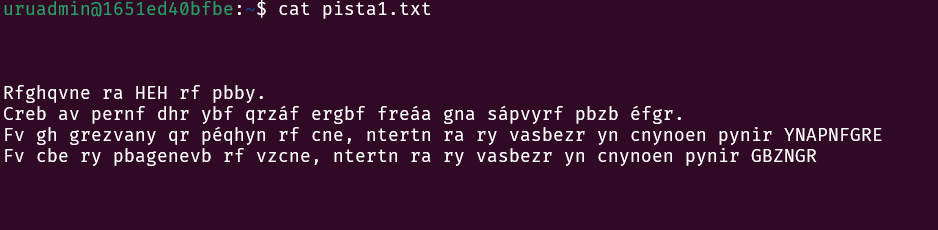
\includegraphics[width=\textwidth]{pista1.png}
  \caption{Contenido del archivo \texttt{pista1.txt}}
  \label{fig:pista1}
\end{figure}

Por ser uno de los cifrados clásicos más comunes, se intenta descifrar el mensaje utilizando \texttt{rot13}, que puede lograrse fácilmente en linux con el comando \texttt{tr}. El comando utilizado será el siguiente.

\begin{verbatim}
  cat pista1.txt | tr 'A-Za-z' 'N-ZA-Mn-za-m'
\end{verbatim}

El primer argumento del comando \texttt{tr 'A-Za-z' 'N-ZA-Mn-za-m'} especifica que se aplicará a cualquier caracter alfabético en mayúscula o minúscula, y el segundo argumento especifica que se reemplazará por el caracter que se encuentra 13 posiciones adelante en el alfabeto. El resultado de la ejecución de este comando se muestra en la Figura \ref{fig:pista1_decoded}.

\begin{figure}[ht!]
  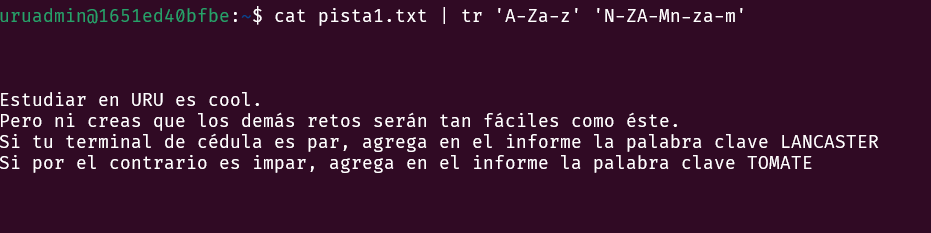
\includegraphics[width=\textwidth]{pista1_decoded.png}
  \caption{Contenido del archivo \texttt{pista1.txt} decodificado}
  \label{fig:pista1_decoded}
\end{figure}

La decodificación de este archivo fue muy sencilla, ya que se utilizó un cifrado muy común y poco seguro. Estas técnicas criptográficas no se consideran nada seguras, y la información cifrada con estas es prácticamente pública. Siguendo las indicaciones de la pista uno, se agrega la palabra indicada en este informe: \texttt{LANCASTER}.

\subsection{Archivo 2: \texttt{pista2}}

Se procedió a imprimir el contenido del archivo \texttt{pista2} y se obtuvo el resultado que se muestra en la Figura \ref{fig:pista2}. Se puede ver que el contenido es una cadena de texto cifrada, pero no se puede inferir el tipo de cifrado utilizado con tanta facilidad.

\begin{figure}[ht!]
  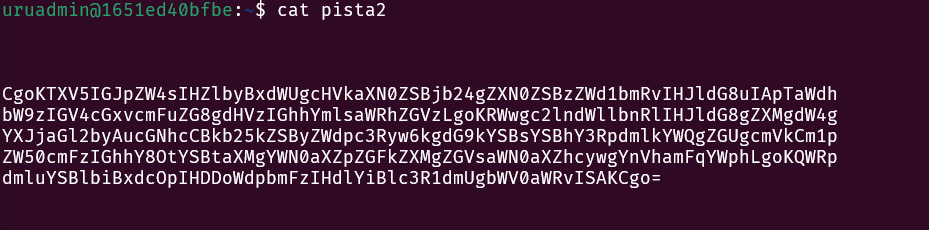
\includegraphics[width=\textwidth]{pista2.png}
  \caption{Contenido del archivo \texttt{pista2}}
  \label{fig:pista2}
\end{figure}

Esta secuencia de caracteres podría estar cifrada con algún tipo de algoritmo simétrico o asimétrico, para lo cual se necesitaría una llave de desencriptación. Sin embargo, como la presentación del desafío estableció que la información necesaria se encuentra en el archivo \texttt{/home/uruadmin}, y siguiendo el orden de las pistas, aún no se ha encontrado ninguna llave, se procede a intentar decodificar el mensaje utilizando el comando \texttt{base64 --decode}, ya que no requiere de una llave de desencriptación. El comando utilizado será el siguiente.

\begin{verbatim}
  cat pista2 | base64 --decode
\end{verbatim}

El comando \texttt{base64 --decode} decodifica la cadena de texto que se le pasa como argumento, y el resultado de la ejecución de este comando se muestra en la Figura \ref{fig:pista2_decoded}.

\begin{figure}[ht!]
  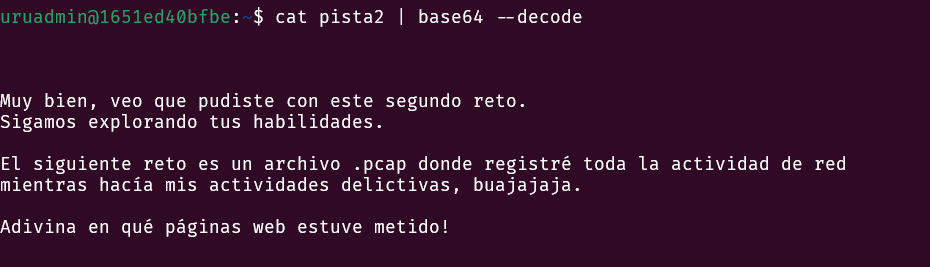
\includegraphics[width=\textwidth]{pista2_decoded.png}
  \caption{Contenido del archivo \texttt{pista2} decodificado}
  \label{fig:pista2_decoded}
\end{figure}

El resultado indica el objetivo para la pista tres, que será determinar los sitios web a los que accedió el atacante, y que están registrados en el archivo \texttt{pista3.pcap}.

\subsection{Archivo 3: \texttt{pista3.pcap}}

Como se conoce que el archivo \texttt{pista3.pcap} contiene un formato específico de captura de tráfico de red, utilizar \texttt{cat} para imprimir su contenido no será útil. En su lugar, se utilizará el comando \texttt{tcpdump} para analizar el tráfico de red y obtener la información necesaria.

Se quieren obtener los sitios web a los que accedió el atacante, por lo que se obtienen solo las peticiones HTTP que se realizaron en el archivo \texttt{pista3.pcap}. Utilizando el manual de \texttt{tcpdump} \cite{thetcpdumpgroup_2020_tcpdump1} podemos encontrar el siguiente
comando, que nos proporciona el resultado que necesitamos.

\begin{verbatim}
  sudo tcpdump 'tcp port 80 and (((ip[2:2] - ((ip[0]&0xf)<<2)) 
  
  - ((tcp[12]&0xf0)>>2)) != 0)'
\end{verbatim}

En este caso, el comando, el filtro \texttt{'tcp port 80'} se encarga de filtrar los paquetes que utilizan el protocolo TCP y el puerto 80 con IPv4, que es el puerto por defecto para el protocolo HTTP. El filtro \texttt{'(((ip[2:2] - ((ip[0]\&0xf)<<2)) - ((tcp[12]\&0xf0)>>2)) != 0'} se encarga de filtrar los paquetes que contengan datos. El resultado de la ejecución de este comando es extremadamente largo, por lo que se muestra solo una parte en la Figura \ref{fig:pista3}.

\begin{figure}[ht!]
  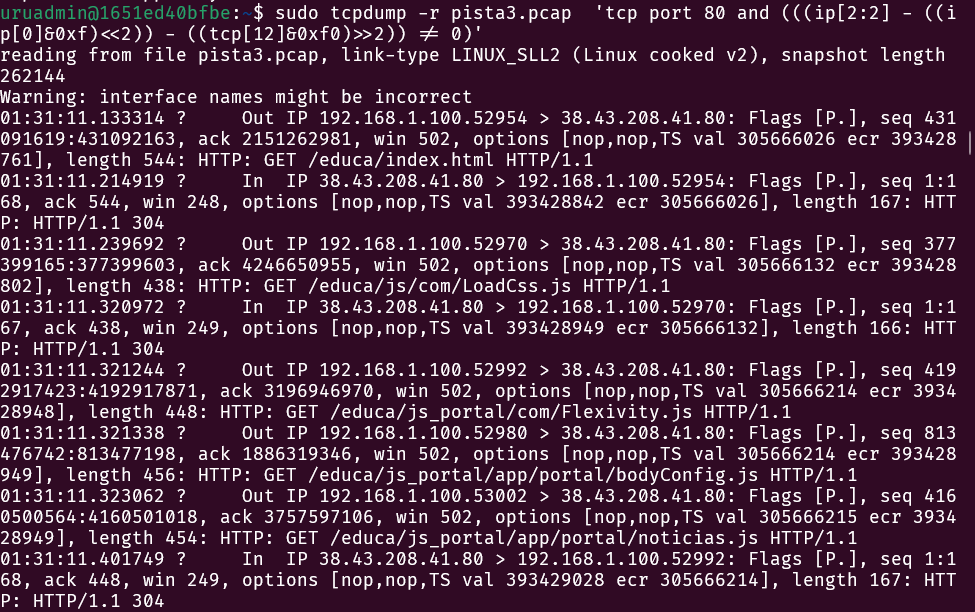
\includegraphics[width=\textwidth]{pista3.png}
  \caption{Extracto del contenido de \texttt{pista3.pcap}}
  \label{fig:pista3}
\end{figure}

En la salida, se puede observar que el atacante accedió únicamente a un sitio web alojado en la direccion IP \texttt{38.43.208.41}. Se puede intentar hacer una búsqueda inversa de la dirección IP para obtener el nombre del dominio, pero la máquina no cuenta con ninguna herramienta para lograr esto, como \texttt{nslookup} o \texttt{dig}. Sin embargo, se puede intentar acceder a la dirección IP en un navegador web para obtener el nombre del dominio. Al acceder a la dirección IP en un navegador web, se obtiene el resultado que se muestra en la Figura \ref{fig:web}.


\begin{figure}[ht!]
  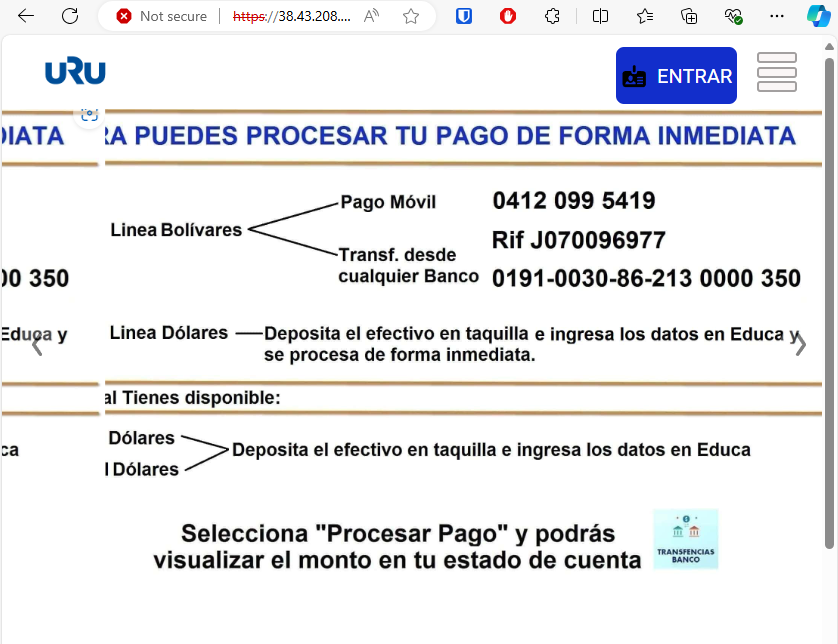
\includegraphics[width=\textwidth]{web.png}
  \caption{Acceso al sitio web alojado en la dirección IP \texttt{38.43.208.41}}
  \label{fig:web}
\end{figure}

En este caso, no es necesario realizar una búsqueda inversa de la dirección IP, ya que se puede observar que es el sitio web del panel de estudiantes de la Universidad Rafael Urdaneta, alojado en \texttt{uru.insiemp.com}. El atacante estuvo accediendo a este sitio web para llevar a cabo sus actividades maliciosas. El atacante únicamente realizó peticiones HTTP GET, por lo que no se puede determinar con exactitud qué actividades realizó el atacante en el sitio web.

Sin embargo, realizando un análisis de tráfico al ingresar manualmente al sitio web, obtenemos un resultado muy similar al que se muestra en la Figura \ref{fig:web}. Un extracto de este se muestra en la Figura \ref{fig:web_manual}. Esto indica que el atacante únicamente ingresó en la página principal del sitio web, y no realizó ninguna acción adicional.

\begin{figure}[ht!]
  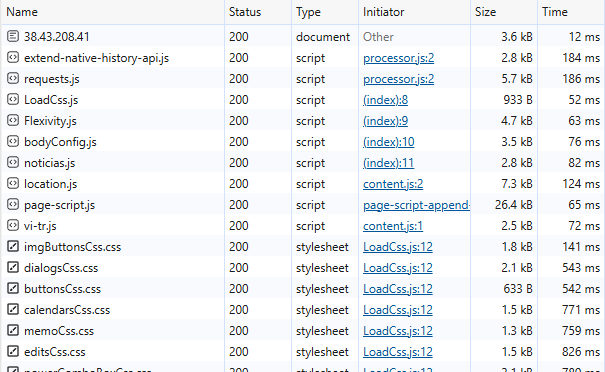
\includegraphics[width=\textwidth]{web_manual.png}
  \caption{Acceso manual al sitio web alojado en la dirección IP \texttt{38.43.208.41}}
  \label{fig:web_manual}
\end{figure}

\subsection{Archivo 4: \texttt{pista4}}

Se muestra el contenido el archivo \texttt{pista4} en la Figura \ref{fig:pista4}.

\begin{figure}[ht!]
  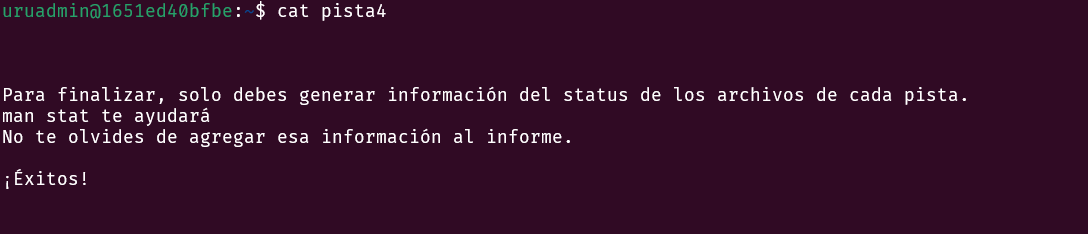
\includegraphics[width=\textwidth]{pista4.png}
  \caption{Contenido del archivo \texttt{pista4}}
  \label{fig:pista4}
\end{figure}

Como se establece en el archivo, únicamente debemos generar información del estatus de los archivos de cada pista. Para esto, se utiliza el comando \texttt{stat} y se obtiene la información deseada. Las figuras \ref{fig:pista1_stat}, \ref{fig:pista2_stat}, \ref{fig:pista3_stat} y \ref{fig:pista4_stat} muestran la información de los archivos \texttt{pista1.txt}, \texttt{pista2}, \texttt{pista3.pcap} y \texttt{pista4} respectivamente.

\begin{figure}[ht!]
  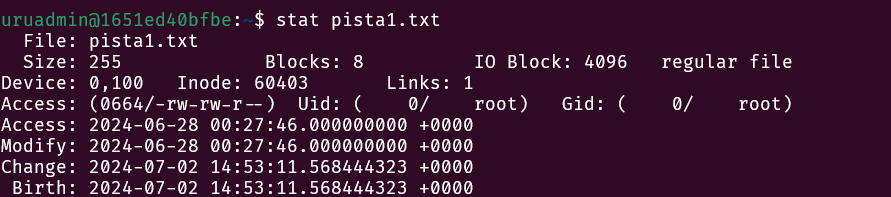
\includegraphics[width=\textwidth]{pista1_stat.png}
  \caption{Estatus del archivo \texttt{pista1.txt}}
  \label{fig:pista1_stat}
\end{figure}

\begin{figure}[ht!]
  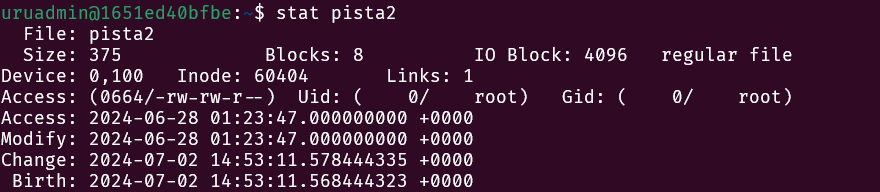
\includegraphics[width=\textwidth]{pista2_stat.png}
  \caption{Estatus del archivo \texttt{pista2}}
  \label{fig:pista2_stat}
\end{figure}

\begin{figure}[ht!]
  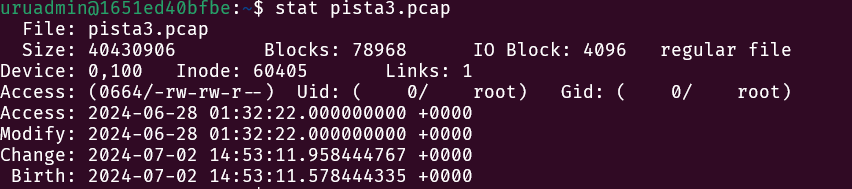
\includegraphics[width=\textwidth]{pista3_stat.png}
  \caption{Estatus del archivo \texttt{pista3.pcap}}
  \label{fig:pista3_stat}
\end{figure}

\begin{figure}[ht!]
  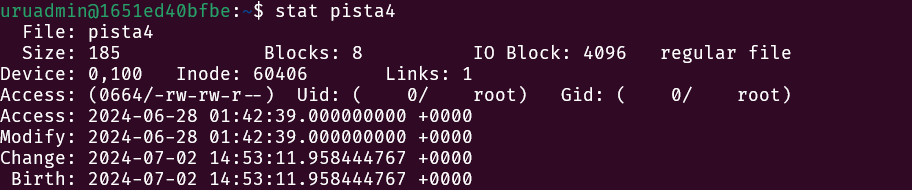
\includegraphics[width=\textwidth]{pista4_stat.png}
  \caption{Estatus del archivo \texttt{pista4}}
  \label{fig:pista4_stat}
\end{figure}

\section{Conclusión}

Durante la ejecución de este desafío, se utilizaron distintas técnicas de análisis criptográfico y de análisis de paquetes para realizar un análisis forense digital de la máquina \texttt{URU-Challenge-2}. Uno por uno, se obtuvo la informacion contenida en los archivos, y se trazó la ruta de acción del atacante.

El primer archivo, el uso de un cifrado rot13 hizo muy sencillo obtener la información necesaria. En la actualidad, las técnicas de cifrado clásicas no son seguras, y siempre se debe utilizar cifrados modernos y seguros, con una clave de cifrado robusta.

El segundo archivo, el uso de base64 para codificar la información, también fue sencillo de decodificar. \texttt{base64} es un algoritmo de codificación muy común, y se utiliza para codificar información binaria en texto ASCII. Sin embargo, no es un algoritmo de cifrado, y no se debe utilizar para proteger información sensible.

El tercer archivo, el análisis de tráfico de red, fue un poco más complicado, ya que se necesitó utilizar \texttt{tcpdump} para analizar el tráfico de red y obtener la información necesaria. El manual de \texttt{tcpdump} \cite{thetcpdumpgroup_2020_tcpdump1} fue de gran ayuda para entender cómo utilizar la herramienta y obtener la información necesaria. La pista dos pidió obtener los sitios web a los que accedió el atacante, por lo que fue mucho más sencillo únicamente analizar las peticiones HTTP contenidas en el archivo \texttt{pista3.pcap}.

El cuarto archivo no contenía información relevante, y únicamente se pidió obtener el estatus de los archivos de cada pista. Para esto, se utilizó el comando \texttt{stat} \cite{kerrisk_2024_stat2} para obtener la información deseada.


\begin{thebibliography}{widestlabel}
  \bibitem{thetcpdumpgroup_2020_tcpdump1}
  The Tcpdump Group. (2020). \textit{tcpdump(1) - Linux}. Recuperado de \url{https://www.tcpdump.org/manpages/tcpdump.1.html}

  \bibitem{kerrisk_2024_stat2}
  Kerrisk, Michael. (2024). \textit{stat(2) - Linux manual page}. Recuperado de
  \url{https://man7.org/linux/man-pages/man2/lstat.2.html}




\end{thebibliography}


\end{document}